\documentclass{article}

\usepackage{amsmath}
\usepackage[usenames,dvipsnames]{color}
\usepackage{multirow}
\usepackage{dot2texi}
\usepackage{algpseudocode}
\algnewcommand{\LineComment}[1]{\State \(\triangleright\) #1}
\algnewcommand{\ShortComment}[1]{\quad \(\triangleright\) #1}

\usepackage{tikz}
\usetikzlibrary{shapes, shapes.multipart, shapes.geometric}
\usetikzlibrary{positioning}

\newcommand*\circled[1]{\tikz[baseline=(char.base)]{
            \node[shape=circle,draw,inner sep=2pt] (char) {#1};}}

\begin{document}

\title{Implementation Report \\ \mbox{ } \\ Model checker for Petri nets}
\author{Philipp Meyer \and Rusl\'{a}n Ledesma-Garza}
% \institute{Technische Universit\"at M\"unchen}
\date{Fri Sep 27 15:30:20 CEST 2013}

\maketitle

\tableofcontents

\iffalse
\begin{verbatim}
- Introduction
  - Diagram of method
- Refinement techniques
  - Trap conditions
  - Subnet trap conditions
  - Empty trap conditions
- State space exploration
- Experiments
  - Trap conditions
    - diagram
    - example: Peterson's
  - Trap and subnet trap conditions
    - diagram
    - example: cyclic net
  - Trap, subnet trap, and empty trap conditions
    - diagram placeholder
    - example: Empty trap condition net
  - State space exploration & trap conditions
- Benchmarks
  - No refinement technique
  - Trap conditions
  - Trap and subnet trap conditions
  - Trap, subnet trap, and empty trap conditions
  - State space exploration and trap conditions
\end{verbatim}
\fi

\section{Introduction}

We report on the implementation of the model checker Pnerf. We
present the design of Pnerf and its corresponding experimental
evaluation.

\section{Design}

Pnerf implements the method in Figure~\ref{fig-method}. Pnerf applies
a given sequence of refinement techniques in each iteration of the
main loop. Each refinement technique tries to produce additional condition
$\delta$ that becomes part of abstraction $C$.

\begin{figure}
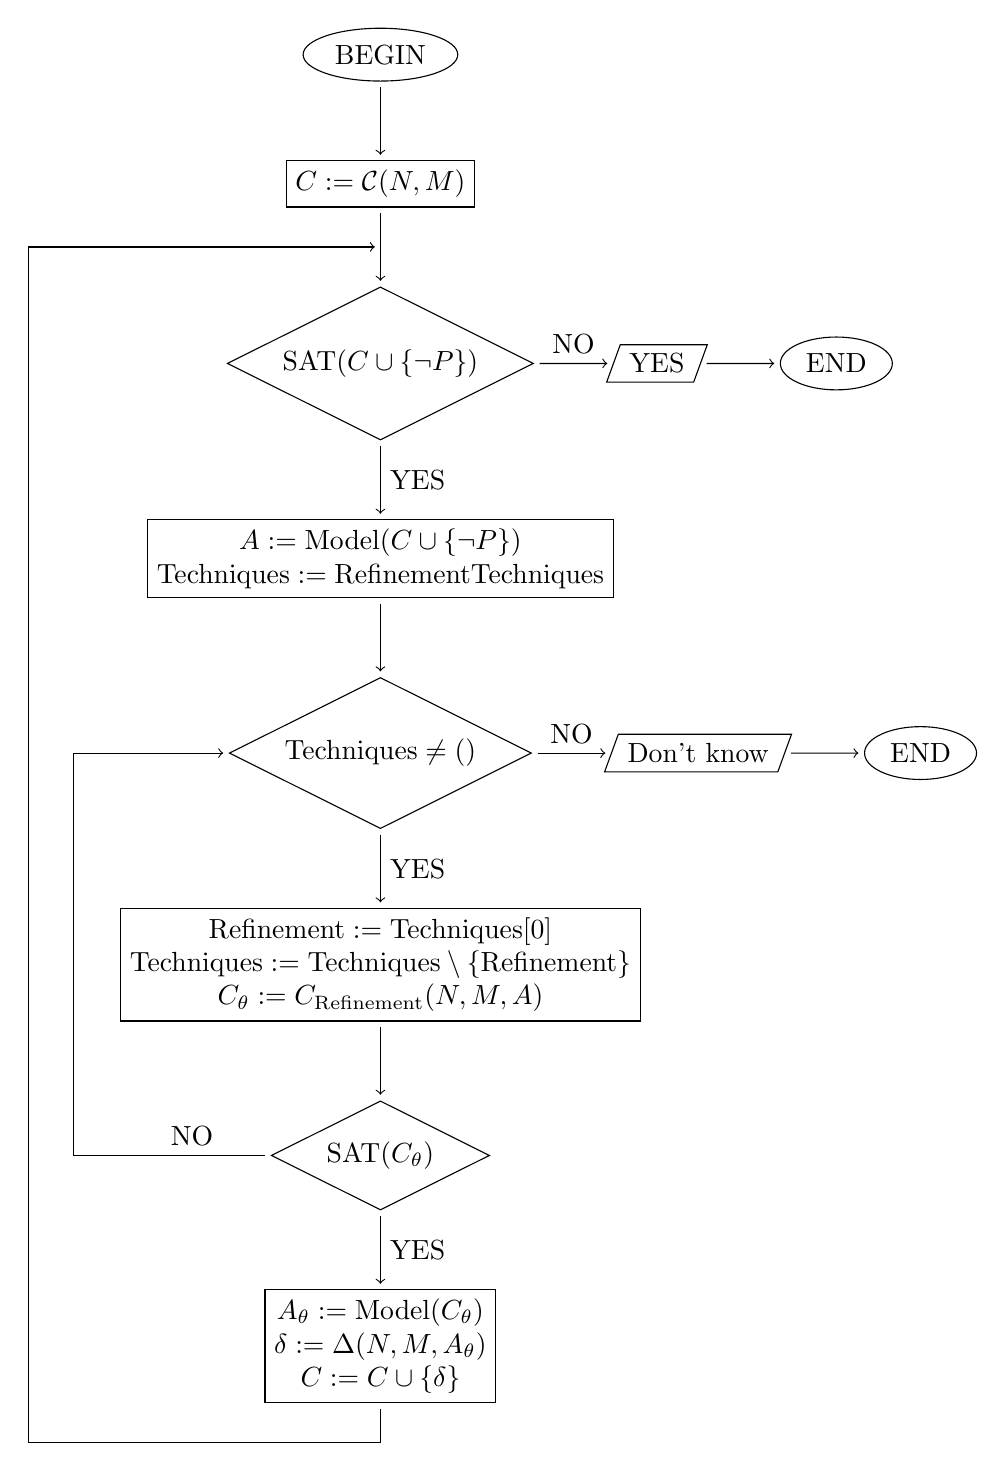
\begin{tikzpicture}[
    state/.style   = {draw, ellipse, aspect=2},
    action/.style  = {draw, rectangle, align=center},
    decision/.style= {draw, diamond, aspect=2, align=center},
    print/.style   = {draw, trapezium, trapezium left angle=70, trapezium right angle=-70},
    edge/.style    = {draw, ->, shorten >=2pt, shorten <=2pt},
  ]
  \node[state] (begin) {BEGIN};
  \node[action, below=of begin] (c) {$C:=\mathcal C(N, M)$};
  \node[decision, below=of c] (satc) {$\text{SAT}(C \cup \{\neg P\})$};
  \node[action, below=of satc] (modelc)
    {$A:=\text{Model}(C \cup \{\neg P\})$ \\
     $\text{Techniques}:=\text{RefinementTechniques}$};
     \node[decision, below=of modelc] (methods) {$\text{Techniques} \neq ()$};
  \node[action, below=of methods] (ctheta)
    {$\text{Refinement} := \text{Techniques}[0]$ \\
     $\text{Techniques}:= \text{Techniques} \setminus \{\text{Refinement}\}$ \\
     $C_{\theta}:=C_{\text{Refinement}}(N, M, A)$};
  \node[decision, below=of ctheta] (satctheta) {$\text{SAT}(C_\theta)$};
  \node[action, below=of satctheta] (modelctheta)
    {$A_\theta:=\text{Model}(C_\theta)$\\
     $\delta:=\Delta(N, M, A_\theta)$\\
     $C:=C \cup \{\delta\}$};
  \node[print, right=of satc] (yes) {YES};
  \node[state, right=of yes] (end1) {END};
  \node[print, right=of methods] (dontknow) {Don't know};
  \node[state, right=of dontknow] (end2) {END};

  \draw (begin) edge[edge] (c);
  \draw (c) edge[edge] coordinate[pos=.5] (edgein) (satc);
  \draw (satc) edge[edge] node[above]{NO} (yes);
  \draw (yes) edge[edge] (end1);
  \draw (satc) edge[edge] node[right]{YES} (modelc);
  \draw (modelc) edge[edge] (methods);
  \draw (methods) edge[edge] node[right]{YES}  (ctheta);
  \draw (methods) edge[edge] node[above]{NO} (dontknow);
  \draw (ctheta) edge[edge] (satctheta);
  \draw (dontknow) edge[edge] (end2);
  \draw (satctheta) edge[edge] node[right]{YES} (modelctheta);
  \draw[edge] (satctheta.west) node[above,xshift=-1cm]{NO}
  -| ([xshift=-2.5cm] satctheta.west) |- (methods.west);
  \draw[edge] (modelctheta.south) -- ([yshift=-0.5cm] modelctheta.south)
  -| ([xshift=-3cm] modelctheta.west) |- (edgein);
\end{tikzpicture}
\caption{Method {\bf Check}}
\label{fig-method}
\end{figure}

\subsection{Refinement techniques}

We implemented the following refinement techniques.

\paragraph{Trap conditions} For a petri net $N$ and an assignment $A$,
find a set $S$ that satisfies
\begin{enumerate}
  \item $S$ is a trap in the net $N$.
  \item $S$ is marked in the initial marking $M_0$.
  \item $S$ is unmarked in the assignment $A$.
\end{enumerate}
For such a set $S$, generate a constraint
$\delta = \left( \sum_{s \in S} s \ge 1 \right)$, ensuring the
trap is marked in any assignment.

\paragraph{Subnet trap conditions} For a petri net $N$ and an assignment $A$,
construct a subnet $N'$ from $N$ that contains only
the transitions that are fired in $A$.
For the net $N'$, find a set $S$ that satisfies
\begin{enumerate}
  \item $S$ is a trap in the subnet $N'$.
  \item $S$ contains a place with an incoming transition in $N'$.
  \item $S$ is unmarked in the assignment $A$.
\end{enumerate}
For such a set $S$, generate a constraint
$\delta = \left( \bigwedge_{t \in T_1} (t > 0) \land
\bigwedge_{t \in T_2} (t = 0) \implies \sum_{s \in S} s \ge 1 \right)$,
where $T_1$ are the transitions fired in $A$ and $T_2$ are the
transitions not fired in $A$. This ensures the trap is marked in the
corresponding subnet.

\paragraph{Empty trap conditions} For a petri net $N$ and an assignment $A$,
find a set $S$ that satisfies
\begin{enumerate}
  \item $S$ is a trap in the net $N$.
  \item $S$ is unmarked in the inital marking $M_0$.
  \item a transition in $S^\bullet$ is fired in $A$
  \item no transition in $^\bullet S \setminus S^\bullet$ is fired in $A$
\end{enumerate}
For such a set $S$, generate a constraint
$\delta = \left( \bigvee_{t \in S^\bullet} (t > 0) \implies
\bigvee_{t \in ^\bullet S \setminus S^\bullet} (t > 0) \right)$
to ensure a proper incoming transition
is fired if an outgoing transition is fired.


\subsection{State space exploration}

Pnerf applies method {\bf Check} in Figure~\ref{fig-method} as a subprocedure of
the state space exploration procedure {\bf Explore} in
Figure~\ref{fig-procedure-explore}.

\begin{figure}[h]
\begin{algorithmic}[1]
\Procedure{Explore}{$N, M_0, P, MaxDepth$}
  \State $Queue \gets ( M_0 )$
  \State $Depth[M_0] \gets 0$
  \State $Visited \gets \emptyset$
  \While {$\neg empty(Queue)$}
    \State $M \gets dequeue(Queue)$
    \State $Visited \gets Visited \cup \{ M \}$
    \If {$Depth[M] = MaxDepth$}
      \State \Return \text{Don't know}
    \EndIf
    \If {$unsafe(M, P)$}
      \State \Return \text{No}
    \EndIf
    \If {$\text{\bf Check}(N, M, P) = \text{Don't know}$}
      \For{$M \rightarrow M_i$}
        \If{$M_i \notin Visited \land M_i \notin Queue$}
          \State $Depth[M_i] \gets Depth[M] + 1$
          \State $enqueue(Queue, M_i)$
        \EndIf
      \EndFor
    \EndIf
  \EndWhile
  \State \Return \text{Yes}
\EndProcedure
\end{algorithmic}
\caption{Procedure {\bf Explore}}
\label{fig-procedure-explore}
\end{figure}


\section{Experiments}

\subsection{Method check}

We applied Pnerf to the set of benchmarks
\verb?benchmarks/given-by-daniel-kroening/?. We applied the following
four configurations for the refinement sequence.
\begin{itemize}
  \item No refinement
  \item \textcolor{OliveGreen}{Trap conditions}
  \item \textcolor{red}{Trap conditions, subnet trap conditions}
  \item \textcolor{blue}{Trap conditions, subnet trap conditions, empty trap conditions}
\end{itemize}
On the benchmark given by Daniel Kroening, we obtained the results in Table~\ref{table-results-method-dk}.
On the benchmark given by mist, we obtained the results in Table~\ref{table-results-method-mist}.

\begin{table}[h]
\begin{center}
  \begin{tabular}{ cc | r | r | r | r | }
    \cline{3-5}
    & & \multicolumn{3}{ c| }{Our tool} \\
    \cline{3-5}
    & & positive & don't know & timeout 10 min &
    \multicolumn{1}{ |c }{} \\ \cline{1-6}
    \multicolumn{1}{ |c| }{\multirow{3}{*}{Mist}} &
    \multicolumn{1}{ |c| }{positive} &
    8 \textcolor{OliveGreen}{8} \textcolor{red}{8} \textcolor{blue}{8} &
    3 \textcolor{OliveGreen}{3} \textcolor{red}{3} \textcolor{blue}{3} &
    0 \textcolor{OliveGreen}{0} \textcolor{red}{0} \textcolor{blue}{0} &
    11 \\ \cline{2-6}
    \multicolumn{1}{ |c  }{} &
    \multicolumn{1}{ |c| }{negative} &
    0 \textcolor{OliveGreen}{0} \textcolor{red}{0} \textcolor{blue}{0} &
    28 \textcolor{OliveGreen}{28} \textcolor{red}{28} \textcolor{blue}{27} &
    0 \textcolor{OliveGreen}{0} \textcolor{red}{0} \textcolor{blue}{1} &
    28 \\ \cline{2-6}
    \multicolumn{1}{ |c  }{} &
    \multicolumn{1}{ |c| }{timeout 1 min} &
    15 \textcolor{OliveGreen}{15} \textcolor{red}{15} \textcolor{blue}{15} &
    23 \textcolor{OliveGreen}{23} \textcolor{red}{19} \textcolor{blue}{16} &
    0 \textcolor{OliveGreen}{0} \textcolor{red}{4} \textcolor{blue}{7} &
    38 \\ \cline{1-6}
    \multicolumn{1}{ c }{} &
    \multicolumn{1}{ c| }{} &
    23 \textcolor{OliveGreen}{23} \textcolor{red}{23} \textcolor{blue}{23} &
    54 \textcolor{OliveGreen}{54} \textcolor{red}{50} \textcolor{blue}{46} &
    0 \textcolor{OliveGreen}{0} \textcolor{red}{4} \textcolor{blue}{8} &
    77 \\ \cline{3-6}
  \end{tabular}
\end{center}
\caption{Results with different configurations of the refinement sequence
  on the benchmarks given by Daniel Kroening}
\label{table-results-method-dk}
\end{table}

\begin{table}[h]
\begin{center}
  \begin{tabular}{ cc | r | r | r | r | }
    \cline{3-5}
    & & \multicolumn{3}{ c| }{Our tool} \\
    \cline{3-5}
    & & positive & don't know & timeout 10 min &
    \multicolumn{1}{ |c }{} \\ \cline{1-6}
    \multicolumn{1}{ |c| }{\multirow{3}{*}{Mist}} &
    \multicolumn{1}{ |c| }{positive} &
    3 \textcolor{OliveGreen}{6} \textcolor{red}{6} \textcolor{blue}{6} &
    3 \textcolor{OliveGreen}{0} \textcolor{red}{0} \textcolor{blue}{0} &
    0 \textcolor{OliveGreen}{0} \textcolor{red}{0} \textcolor{blue}{0} &
    6 \\ \cline{2-6}
    \multicolumn{1}{ |c  }{} &
    \multicolumn{1}{ |c| }{negative} &
    0 \textcolor{OliveGreen}{0} \textcolor{red}{0} \textcolor{blue}{0} &
    0 \textcolor{OliveGreen}{0} \textcolor{red}{0} \textcolor{blue}{0} &
    0 \textcolor{OliveGreen}{0} \textcolor{red}{0} \textcolor{blue}{0} &
    0 \\ \cline{2-6}
    \multicolumn{1}{ |c  }{} &
    \multicolumn{1}{ |c| }{timeout 1 min} &
    0 \textcolor{OliveGreen}{0} \textcolor{red}{0} \textcolor{blue}{0} &
    0 \textcolor{OliveGreen}{0} \textcolor{red}{0} \textcolor{blue}{0} &
    0 \textcolor{OliveGreen}{0} \textcolor{red}{0} \textcolor{blue}{0} &
    0 \\ \cline{1-6}
    \multicolumn{1}{ c }{} &
    \multicolumn{1}{ c| }{} &
    3 \textcolor{OliveGreen}{6} \textcolor{red}{6} \textcolor{blue}{6} &
    3 \textcolor{OliveGreen}{0} \textcolor{red}{0} \textcolor{blue}{0} &
    0 \textcolor{OliveGreen}{0} \textcolor{red}{0} \textcolor{blue}{0} &
    6 \\ \cline{3-6}
  \end{tabular}
\end{center}
\caption{Results with different configurations of the refinement sequence
  on the benchmarks given by mist}
\label{table-results-method-mist}
\end{table}

\subsection{Method explore}

For the purpose of checking the remaining 3 `don't know` benchmarks,
we applied the procedure {\bf Explore} with the following parameters.
\begin{itemize}
  \item \textcolor{WildStrawberry}{Depth = 30, RefinementTechniques=(Trap conditions), timeout=1min}
  \item \textcolor{NavyBlue}{Depth = 10, RefinementTechniques=(Trap conditions), timeout=1min}
  \item \textcolor{orange}{Depth = 10, RefinementTechniques=(Trap conditions), timeout=10min}
\end{itemize}
We obtained the results in Table~\ref{table-results-explore}.

\begin{table}[h]
\begin{center}
  \begin{tabular}{ cc | r | r | r | r | r | }
    \cline{3-6}
    & & \multicolumn{4}{ c| }{Our tool} \\
    \cline{3-6}
    & & positive & negative & don't know & timeout &
    \multicolumn{1}{ |c }{} \\ \cline{1-7}
    \multicolumn{1}{ |c| }{\multirow{3}{*}{Mist}} &
    \multicolumn{1}{ |c| }{positive} &
    \textcolor{WildStrawberry}{10} \textcolor{NavyBlue}{8} \textcolor{orange}{8} &
    \textcolor{WildStrawberry}{0} \textcolor{NavyBlue}{0} \textcolor{orange}{0} &
    \textcolor{WildStrawberry}{1} \textcolor{NavyBlue}{3} \textcolor{orange}{3} &
    \textcolor{WildStrawberry}{0} \textcolor{NavyBlue}{0} \textcolor{orange}{0} &
    11 \\ \cline{2-7}
    \multicolumn{1}{ |c  }{} &
    \multicolumn{1}{ |c| }{negative} &
    \textcolor{WildStrawberry}{0} \textcolor{NavyBlue}{0} \textcolor{orange}{0} &
    \textcolor{WildStrawberry}{8} \textcolor{NavyBlue}{8} \textcolor{orange}{10} &
    \textcolor{WildStrawberry}{0} \textcolor{NavyBlue}{6} \textcolor{orange}{18} &
    \textcolor{WildStrawberry}{20} \textcolor{NavyBlue}{14} \textcolor{orange}{0} &
    28 \\ \cline{2-7}
    \multicolumn{1}{ |c  }{} &
    \multicolumn{1}{ |c| }{timeout 1 min} &
    \textcolor{WildStrawberry}{15} \textcolor{NavyBlue}{15} \textcolor{orange}{15} &
    \textcolor{WildStrawberry}{0} \textcolor{NavyBlue}{0} \textcolor{orange}{0} &
    \textcolor{WildStrawberry}{0} \textcolor{NavyBlue}{1} \textcolor{orange}{5} &
    \textcolor{WildStrawberry}{23} \textcolor{NavyBlue}{22} \textcolor{orange}{18} &
    38 \\ \cline{1-7}
    \multicolumn{1}{ c }{} &
    \multicolumn{1}{ c| }{} &
    \textcolor{WildStrawberry}{25} \textcolor{NavyBlue}{23} \textcolor{orange}{23} &
    \textcolor{WildStrawberry}{8} \textcolor{NavyBlue}{8} \textcolor{orange}{10} &
    \textcolor{WildStrawberry}{1} \textcolor{NavyBlue}{10} \textcolor{orange}{26} &
    \textcolor{WildStrawberry}{43} \textcolor{NavyBlue}{36} \textcolor{orange}{18} &
    77 \\ \cline{3-7}
  \end{tabular}
\end{center}
\caption{Results with the procedure {\bf Explore}}
\label{table-results-explore}
\end{table}

\subsection{Comparision of mist and bfc}

We compared the tool mist with the tool bfc from http://www.cprover.org/bfc/.
We obtained the results in Table~\ref{table-results-mist-bfc}.

\begin{table}[h]
\begin{center}
  \begin{tabular}{ cc | r | r | r | r | }
    \cline{3-5}
    & & \multicolumn{3}{ c| }{Mist} \\
    \cline{3-5}
    & & positive & negative & timeout 1 min &
    \multicolumn{1}{ |c }{} \\ \cline{1-6}
    \multicolumn{1}{ |c| }{\multirow{3}{*}{Bfc}} &
    \multicolumn{1}{ |c| }{positive} &
    11 &  0 & 15 & 26 \\ \cline{2-6}
    \multicolumn{1}{ |c  }{} &
    \multicolumn{1}{ |c| }{negative} &
     0 & 28 & 23 & 51 \\ \cline{2-6}
    \multicolumn{1}{ |c  }{} &
    \multicolumn{1}{ |c| }{timeout 1 min} &
     0 &  0 &  0 &  0 \\ \cline{1-6}
    \multicolumn{1}{ c }{} &
    \multicolumn{1}{ c| }{} &
    11 & 28 & 38 & 77 \\ \cline{3-6}
  \end{tabular}
\end{center}
\caption{Results of comparing mist and bfc}
\label{table-results-mist-bfc}
\end{table}

\subsection{Method check and explore}

We modified the method {\bf Explore} to not call {\bf Check} on each marking
and combined the method {\bf Check} on the initial marking with
a call to the modified {\bf Explore} if {\bf Check} returns don't know.

The parameters were
\begin{itemize}
  \item \textcolor{BrickRed}{RefinementTechniques=(), Depth = 100, timeout=1min}
  \item \textcolor{NavyBlue}{RefinementTechniques=(), Depth = 100, timeout=10min}
\end{itemize}
After comparing the results with bfc, we obtained the results in Table~\ref{table-results-check-explore}.

\begin{table}[h]
\begin{center}
  \begin{tabular}{ cc | r | r | r | r | r | }
    \cline{3-6}
    & & \multicolumn{4}{ c| }{Our tool} \\
    \cline{3-6}
    & & positive & negative & don't know & timeout &
    \multicolumn{1}{ |c }{} \\ \cline{1-7}
    \multicolumn{1}{ |c| }{\multirow{3}{*}{Bfc}} &
    \multicolumn{1}{ |c| }{positive} &
    \textcolor{BrickRed}{26} \textcolor{NavyBlue}{26} &
    \textcolor{BrickRed}{0} \textcolor{NavyBlue}{0} &
    \textcolor{BrickRed}{0} \textcolor{NavyBlue}{0} &
    \textcolor{BrickRed}{0} \textcolor{NavyBlue}{0} &
    26 \\ \cline{2-7}
    \multicolumn{1}{ |c  }{} &
    \multicolumn{1}{ |c| }{negative} &
    \textcolor{BrickRed}{0} \textcolor{NavyBlue}{0} &
    \textcolor{BrickRed}{34} \textcolor{NavyBlue}{39} &
    \textcolor{BrickRed}{0} \textcolor{NavyBlue}{0} &
    \textcolor{BrickRed}{17} \textcolor{NavyBlue}{12} &
    51 \\ \cline{2-7}
    \multicolumn{1}{ |c  }{} &
    \multicolumn{1}{ |c| }{timeout 1 min} &
    \textcolor{BrickRed}{0} \textcolor{NavyBlue}{0} &
    \textcolor{BrickRed}{0} \textcolor{NavyBlue}{0} &
    \textcolor{BrickRed}{0} \textcolor{NavyBlue}{0} &
    \textcolor{BrickRed}{0} \textcolor{NavyBlue}{0} &
    38 \\ \cline{1-7}
    \multicolumn{1}{ c }{} &
    \multicolumn{1}{ c| }{} &
    \textcolor{BrickRed}{26} \textcolor{NavyBlue}{26} &
    \textcolor{BrickRed}{34} \textcolor{NavyBlue}{39} &
    \textcolor{BrickRed}{0} \textcolor{NavyBlue}{0} &
    \textcolor{BrickRed}{17} \textcolor{NavyBlue}{12} &
    77 \\ \cline{3-7}
  \end{tabular}
\end{center}
\caption{Results with the procedure {\bf Check} and procedure {\bf Explore}}
\label{table-results-check-explore}
\end{table}

\subsection{State equation with real numbers}

We modified the method {\bf Check} to use real numbers for the
solution of the state equation and ran it without any refinement techniques.
We obtained the results in Table~\ref{table-results-check-real}.

\begin{table}[h]
\begin{center}
  \begin{tabular}{ cc | r | r | r | r | r | }
    \cline{3-6}
    & & \multicolumn{4}{ c| }{Our tool} \\
    \cline{3-6}
    & & positive & negative & don't know & timeout &
    \multicolumn{1}{ |c }{} \\ \cline{1-7}
    \multicolumn{1}{ |c| }{\multirow{3}{*}{Bfc}} &
    \multicolumn{1}{ |c| }{positive} &
    23 &  0 &  3 &  0 & 26 \\ \cline{2-7}
    \multicolumn{1}{ |c  }{} &
    \multicolumn{1}{ |c| }{negative} &
     0 &  0 & 51 &  0 & 51 \\ \cline{2-7}
    \multicolumn{1}{ |c  }{} &
    \multicolumn{1}{ |c| }{timeout 1 min} &
     0 &  0 &  0 &  0 &  0 \\ \cline{1-7}
    \multicolumn{1}{ c }{} &
    \multicolumn{1}{ c| }{} &
    23 &  0 & 54 &  0 & 77 \\ \cline{3-7}
  \end{tabular}
\end{center}
\caption{Results with the procedure {\bf Check} with real numbers}
\label{table-results-check-real}
\end{table}

\subsection{Observations}

The compiled results of all methods are shown in table \ref{table-results-compiled}.
\begin{table}[h]
\begin{center}
  \begin{tabular}{ | p{5cm} | r | r | r | r | }
    \hline
    Method & positive & negative & don't know & timeout \\
    \hline
    State equation with real numbers & 23 &  0 & 54 &  0 \\
    State equation with integers     & 23 &  0 & 54 &  0  \\
    \hline
    RefinementTechniques = ( TrapConditions ) & 23 &  0 & 54 &  0 \\
    RefinementTechniques = ( TrapConditions, SubnetTrapConditions ) &
    23 &  0 & 50 &  4 \\
    RefinementTechniques = ( TrapConditions, SubnetTrapConditions, EmptyTrapConditions ) &
    23 &  0 & 46 &  8 \\
    \hline
    State space exploration with check, D=30, t=1min  & 25 &  8 &  1 &  43 \\
    State space exploration with check, D=10, t=1min  & 23 &  8 & 10 &  36 \\
    State space exploration with check, D=10, t=10min & 23 & 10 & 26 &  18 \\
    \hline
    Check + State space exploration without check, D=100, t=1min & 26 & 34 & 0 &  17 \\
    Check + State space exploration without check, D=100, t=1min & 26 & 39 & 0 &  12 \\
    \hline
    Mist tool & 11 & 28 & 0 & 38 \\
    Bfc tool  & 26 & 51 & 0 &  0 \\
    \hline
  \end{tabular}
\end{center}
\caption{Compiled results}
\label{table-results-compiled}
\end{table}

From table \ref{table-results-mist-bfc}, we see that there are no contradictions between mist and bfc.

From table \ref{table-results-check-explore}, we see that there are no contradictions between our tool and bfc. Further our tool returns a positive result for all the positive benchmarks.

\section{Experimental setups}

\subsection{Trap conditons}

The corresponding method appears in Figure~\ref{fig-method-trap}.

\begin{figure}[h]
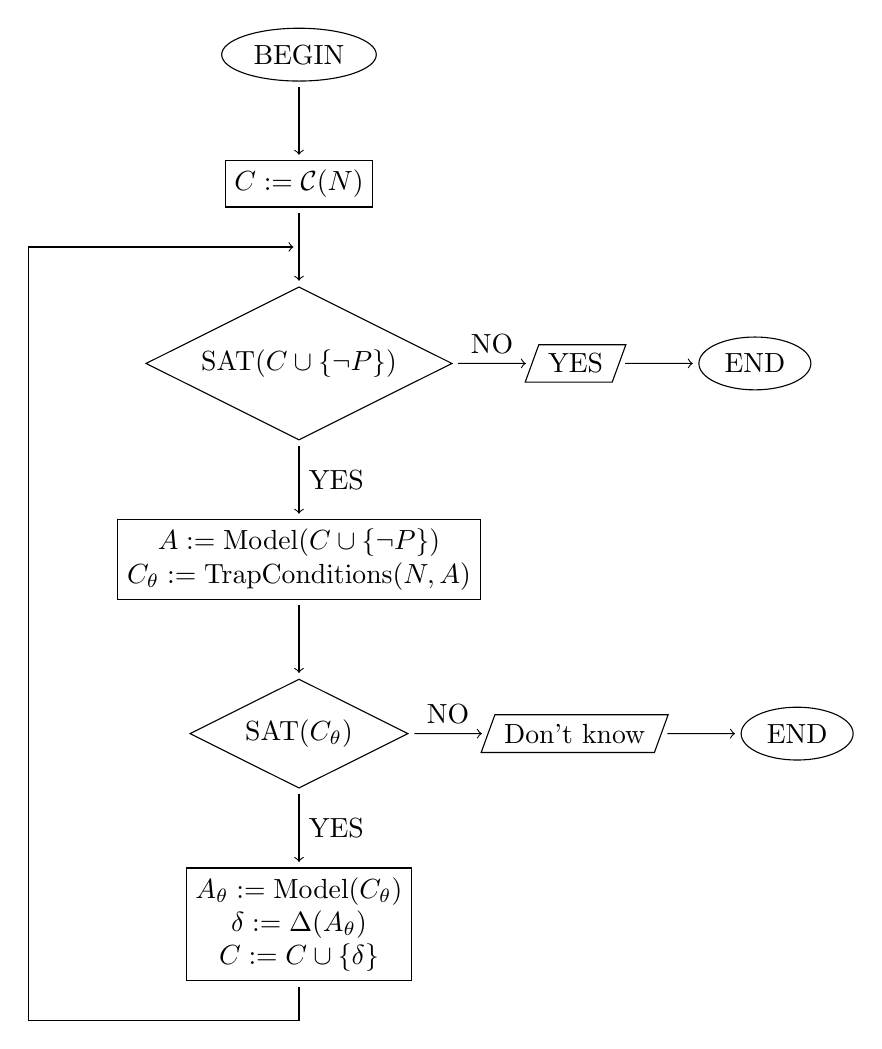
\begin{tikzpicture}[
    state/.style   = {draw, ellipse, aspect=2},
    action/.style  = {draw, rectangle, align=center},
    decision/.style= {draw, diamond, aspect=2, align=center},
    print/.style   = {draw, trapezium, trapezium left angle=70, trapezium right angle=-70},
    edge/.style    = {draw, ->, shorten >=2pt, shorten <=2pt},
  ]
  \node[state] (begin) {BEGIN};
  \node[action, below=of begin] (c) {$C:=\mathcal C(N)$};
  \node[decision, below=of c] (satc) {$\text{SAT}(C \cup \{\neg P\})$};
  \node[action, below=of satc] (modelc) {$A:=\text{Model}(C \cup \{\neg P\})$\\
                                   $C_{\theta}:=\text{TrapConditions}(N, A)$};
  \node[decision, below=of modelc] (satctheta) {$\text{SAT}(C_\theta)$};
  \node[action, below=of satctheta] (modelctheta) {$A_\theta:=\text{Model}(C_\theta)$\\
                                        $\delta:=\Delta(A_\theta)$\\
                                        $C:=C \cup \{\delta\}$};
  \node[print, right=of satc] (yes) {YES};
  \node[print, right=of satctheta] (dontknow) {Don't know};
  \node[state, right=of yes] (end1) {END};
  \node[state, right=of dontknow] (end2) {END};

  \draw (begin) edge[edge] (c);
  \draw (c) edge[edge] coordinate[pos=.5] (edgein) (satc);
  \draw (satc) edge[edge] node[above]{NO} (yes);
  \draw (yes) edge[edge] (end1);
  \draw (satc) edge[edge] node[right]{YES} (modelc);
  \draw (modelc) edge[edge] (satctheta);
  \draw (satctheta) edge[edge] node[above]{NO} (dontknow);
  \draw (dontknow) edge[edge] (end2);
  \draw (satctheta) edge[edge] node[right]{YES} (modelctheta);
  \draw[edge] (modelctheta.south) -- ([yshift=-0.5cm] modelctheta.south)
  -| ([xshift=-2cm] modelctheta.west) |- (edgein);
\end{tikzpicture}
\caption{Method {\bf Check} with RefinementTechniques=({\bf Trap
    conditions})}
\label{fig-method-trap}
\end{figure}

\subsubsection{Example: Peterson's Algorithm}

Taken from Javier's notes on petri nets
(http://www7.in.tum.de/um/courses/petri/SS2013/PNSkript.pdf, p. 16).

\paragraph{Constraints $C_0$}

\begin{alignat*}{15}
&& p_1 &{}={}& 1
  &{}-{}& u_1 &     &     &     &     &     &     &     &     &{}+{}& u_6 
  &     &     &     &     &     &     &     &     &     &     &     &     \\
&& p_2 &{}={}& 0
  &{}+{}& u_1 &{}-{}& u_2 &{}-{}& u_3 &     &     &     &     &     &     
  &     &     &     &     &     &     &     &     &     &     &     &     \\
&& p_3 &{}={}& 0
  &     &     &{}+{}& u_2 &{}+{}& u_3 &{}-{}& u_4 &{}-{}& u_5 &     &     
  &     &     &     &     &     &     &     &     &     &     &     &     \\
&& p_4 &{}={}& 0
  &     &     &     &     &     &     &{}+{}& u_4 &{}+{}& u_5 &{}-{}& u_6
  &     &     &     &     &     &     &     &     &     &     &     &     \\
&& q_1 &{}={}& 1
  &     &     &     &     &     &     &     &     &     &     &     &     
  &{}-{}& v_1 &     &     &     &     &     &     &     &     &{}+{}& v_6 \\
&& q_2 &{}={}& 0
  &     &     &     &     &     &     &     &     &     &     &     &    
  &{}+{}& v_1 &{}-{}& v_2 &{}-{}& v_3 &     &     &     &     &     &     \\
&& q_3 &{}={}& 0
  &     &     &     &     &     &     &     &     &     &     &     &     
  &     &     &{}+{}& v_2 &{}+{}& v_3 &{}-{}& v_4 &{}-{}& v_5 &     &     \\
&& q_4 &{}={}& 0
  &     &     &     &     &     &     &     &     &     &     &     &     
  &     &     &     &     &     &     &{}+{}& v_4 &{}+{}& v_5 &{}-{}& v_6 \\
&& (m_1=f) &{}={}& 1
  &{}-{}& u_1 &     &     &     &     &     &     &     &     &{}+{}& u_6     
  &     &     &     &     &     &     &     &     &     &     &     &     \\
&& (m_1=t) &{}={}& 0
  &{}+{}& u_1 &     &     &     &     &     &     &     &     &{}-{}& u_6     
  &     &     &     &     &     &     &     &     &     &     &     &     \\
&& (m_2=f) &{}={}& 1
  &     &     &     &     &     &     &     &     &     &     &     &     
  &{}-{}& v_1 &     &     &     &     &     &     &     &     &{}+{}& v_6 \\    
&& (m_2=t) &{}={}& 0
  &     &     &     &     &     &     &     &     &     &     &     &     
  &{}+{}& v_1 &     &     &     &     &     &     &     &     &{}-{}& v_6 \\    
&& (hold=1) &{}={}& 1
  &     &     &{}+{}& u_2 &     &     &     &     &     &     &     &     
  &     &     &     &     &{}-{}& v_3 &     &     &     &     &     &     \\
&& (hold=2) &{}={}& 0
  &     &     &{}-{}& u_2 &     &     &     &     &     &     &     &     
  &     &     &     &     &{}+{}& v_3 &     &     &     &     &     &     \\
&& p_4 &{}\ge{}& 1 \\
&& q_4 &{}\ge{}& 1 \\
&\forall p \in S \cup T:& p &{}\ge{}& 0
\end{alignat*}

\begin{align*}
  \delta_1 &= p_3 \lor q_2 \lor (m_2=f) \lor (hold=2) \\
  \delta_2 &= p_2 \lor q_3 \lor (m_1=f) \lor (hold=1)
\end{align*}

\paragraph{$A_1$}

\begin{align*}
  p_1 &= 0 \\
  p_2 &= 0 \\
  p_3 &= 0 \\
  p_4 &= 1 \\
  q_1 &= 0 \\
  q_2 &= 0 \\
  q_3 &= 0 \\
  q_4 &= 1 \\
  (m_1=f) &= 0 \\
  (m_1=t) &= 1 \\
  (m_2=f) &= 0 \\
  (m_2=t) &= 1 \\
  (hold=1) &= 1 \\
  (hold=2) &= 0 \\
  u_1 &= 1 \\
  u_2 &= 0 \\
  u_3 &= 1 \\
  u_4 &= 0 \\
  u_5 &= 1 \\
  u_6 &= 0 \\
  v_1 &= 1 \\
  v_2 &= 1 \\
  v_3 &= 0 \\
  v_4 &= 1 \\
  v_5 &= 0 \\
  v_6 &= 0
\end{align*}

\paragraph{$A_2$}

\begin{align*}
  p_1 &= 0 \\
  p_2 &= 0 \\
  p_3 &= 0 \\
  p_4 &= 1 \\
  q_1 &= 0 \\
  q_2 &= 0 \\
  q_3 &= 0 \\
  q_4 &= 1 \\
  (m_1=f) &= 0 \\
  (m_1=t) &= 1 \\
  (m_2=f) &= 0 \\
  (m_2=t) &= 1 \\
  (hold=1) &= 0 \\
  (hold=2) &= 1 \\
  u_1 &= 1 \\
  u_2 &= 1 \\
  u_3 &= 0 \\
  u_4 &= 0 \\
  u_5 &= 1 \\
  u_6 &= 0 \\
  v_1 &= 2 \\
  v_2 &= 0 \\
  v_3 &= 2 \\
  v_4 &= 0 \\
  v_5 &= 2 \\
  v_6 &= 1
\end{align*}

\paragraph{$A_{\theta 1}$}
\begin{align*}
  p_1 &= 0 \\
  p_2 &= 0 \\
  p_3 &= 1 \\
  p_4 &= 0 \\
  q_1 &= 0 \\
  q_2 &= 1 \\
  q_3 &= 0 \\
  q_4 &= 0 \\
  (m_1=f) &= 0 \\
  (m_1=t) &= 0 \\
  (m_2=f) &= 1 \\
  (m_2=t) &= 0 \\
  (hold=1) &= 0 \\
  (hold=2) &= 1
\end{align*}

\paragraph{$A_{\theta 2}$}
\begin{align*}
  p_1 &= 0 \\
  p_2 &= 1 \\
  p_3 &= 0 \\
  p_4 &= 0 \\
  q_1 &= 0 \\
  q_2 &= 0 \\
  q_3 &= 1 \\
  q_4 &= 0 \\
  (m_1=f) &= 1 \\
  (m_1=t) &= 0 \\
  (m_2=f) &= 0 \\
  (m_2=t) &= 0 \\
  (hold=1) &= 1 \\
  (hold=2) &= 0
\end{align*}

\paragraph{$C_\theta$}

\circled{1}
\begin{align*}
  p_1 &\implies o\_u_1 \\
  p_2 &\implies o\_u_2 \land o\_u_3 \\
  p_3 &\implies o\_u_4 \land o\_u_5 \\
  p_4 &\implies o\_u_6 \\
  q_1 &\implies o\_v_1 \\
  q_2 &\implies o\_v_2 \land o\_v_3 \\
  q_3 &\implies o\_v_4 \land o\_v_5 \\
  q_4 &\implies o\_v_6 \\
  (m_1=f) &\implies o\_u_1 \land o\_v_4 \\
  (m_1=t) &\implies o\_u_6 \\
  (m_2=f) &\implies o\_v_1 \land o\_u_4  \\
  (m_2=t) &\implies o\_v_6 \\
  (hold=1) &\implies o\_v_3 \land o\_v_5 \land o\_u_3 \\
  (hold=2) &\implies o\_u_3 \land o\_u_5 \land o\_v_3 \\
  o\_u_1 &\implies (p_2 \lor (m_1=t)) \\
  o\_u_2 &\implies (p_3 \lor (hold=1)) \\
  o\_u_3 &\implies (p_3 \lor (hold=1)) \\
  o\_u_4 &\implies (p_4 \lor (m_2=f)) \\
  o\_u_5 &\implies (p_4 \lor (hold=2)) \\
  o\_u_6 &\implies (p_1 \lor (m_1=f)) \\
  o\_v_1 &\implies (q_2 \lor (m_2=t)) \\
  o\_v_2 &\implies (q_3 \lor (hold=2)) \\
  o\_v_3 &\implies (q_3 \lor (hold=2)) \\
  o\_v_4 &\implies (q_4 \lor (m_1=f)) \\
  o\_v_5 &\implies (p_4 \lor (hold=1)) \\
  o\_v_6 &\implies (q_1 \lor (m_2=f))
\end{align*}
\circled{2}
\begin{align*}
  p_1 \lor q_1 \lor (m_1=f) \lor (m_2=f) \lor (hold=1)
\end{align*}
$\circled{3}_1$
\begin{align*}
  \neg p_4 \land \neg q_4 \land \neg (m_1=t) \land
  \neg (m_2=t) \land \neg (hold=1)
\end{align*}
$\circled{3}_2$
\begin{align*}
  \neg p_4 \land \neg q_4 \land \neg (m_1=t) \land
  \neg (m_2=t) \land \neg (hold=2)
\end{align*}




\subsection{Trap conditions and subnet trap conditions}

The corresponding method appears in Figure~\ref{fig-method-trap-subnet}.

\begin{figure}[h]
  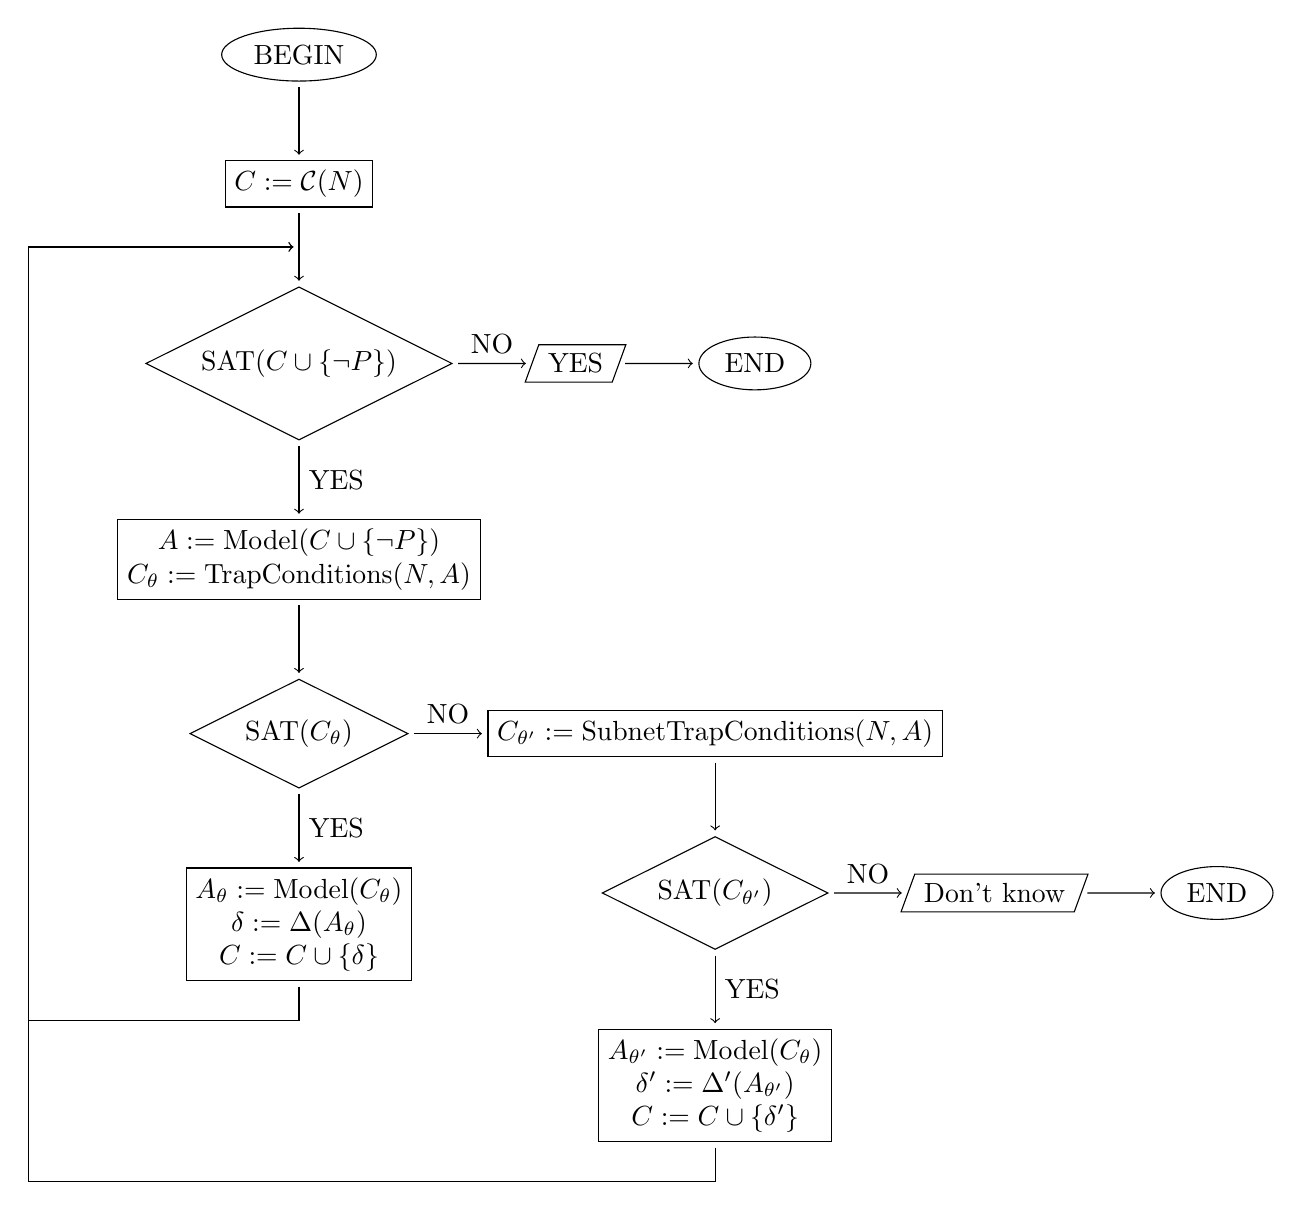
\begin{tikzpicture}[
    state/.style   = {draw, ellipse, aspect=2},
    action/.style  = {draw, rectangle, align=center},
    decision/.style= {draw, diamond, aspect=2, align=center},
    print/.style   = {draw, trapezium, trapezium left angle=70, trapezium right angle=-70},
    edge/.style    = {draw, ->, shorten >=2pt, shorten <=2pt},
    ]
    \node[state] (begin) {BEGIN};
    \node[action, below=of begin] (c) {$C:=\mathcal C(N)$};
    \node[decision, below=of c] (satc) {$\text{SAT}(C \cup \{\neg P\})$};
    \node[action, below=of satc] (modelc) {$A:=\text{Model}(C \cup \{\neg P\})$\\
      $C_{\theta}:=\text{TrapConditions}(N, A)$};
    \node[decision, below=of modelc] (satctheta) {$\text{SAT}(C_\theta)$};
    \node[action, below=of satctheta] (modelctheta) {$A_\theta:=\text{Model}(C_\theta)$\\
      $\delta:=\Delta(A_\theta)$\\
      $C:=C \cup \{\delta\}$};
    \node[print, right=of satc] (yes) {YES};
    \node[action, right=of satctheta] (cthetaprime) {$C_{\theta'}:=\text{SubnetTrapConditions}(N, A)$};
    \node[decision, below=of cthetaprime] (satcthetaprime) {$\text{SAT}(C_{\theta'})$};
    \node[action, below=of satcthetaprime] (modelcthetaprime)
    {$A_{\theta'}:=\text{Model}(C_\theta)$\\
      $\delta':=\Delta'(A_{\theta'})$\\
      $C:=C \cup \{\delta'\}$};
    \node[print, right=of satcthetaprime] (dontknow) {Don't know};
    \node[state, right=of yes] (end1) {END};
    \node[state, right=of dontknow] (end2) {END};

    \draw (begin) edge[edge] (c);
    \draw (c) edge[edge] coordinate[pos=.5] (edgein) (satc);
    \draw (satc) edge[edge] node[above]{NO} (yes);
    \draw (yes) edge[edge] (end1);
    \draw (satc) edge[edge] node[right]{YES} (modelc);
    \draw (modelc) edge[edge] (satctheta);
    \draw (satctheta) edge[edge] node[above]{NO} (cthetaprime);
    \draw (cthetaprime) edge[edge] (satcthetaprime);
    \draw (satcthetaprime) edge[edge] node[above]{NO} (dontknow);
    \draw (dontknow) edge[edge] (end2);
    \draw (satctheta) edge[edge] node[right]{YES} (modelctheta);
    \draw (satcthetaprime) edge[edge] node[right]{YES} (modelcthetaprime);
    \draw[edge] (modelctheta.south) -- ([yshift=-0.5cm] modelctheta.south)
    -| ([xshift=-2cm] modelctheta.west) |- (edgein);
    \draw[edge] (modelcthetaprime.south) -- ([yshift=-0.5cm] modelcthetaprime.south)
    -| ([xshift=-2cm] modelctheta.west) |- (edgein);
  \end{tikzpicture}
  \caption{Method {\bf Check} with RefinementTechniques=({\bf Trap
      conditions}, {\bf Subnet trap conditions})}
  \label{fig-method-trap-subnet}
\end{figure}

\subsubsection{Example: Cyclic net}

Modified version of Stephan Melzer's Dissertation, p. 140.

\begin{dot2tex}[dot,options=-tmath]
\input{cyclic-net.dot}
\end{dot2tex}

\paragraph{Constraints $C_0$}

\begin{alignat*}{6}
&& s_1 &{}={}&   1 &     &     &{}-{}& t_2 &     &     \\
&& s_2 &{}={}&   0 &{}+{}& t_1 &{}-{}& t_2 &     &     \\
&& s_3 &{}={}&   0 &     &     &{}+{}& t_2 &     &     \\
&& s_4 &{}={}&   0 &     &     &     &     &{}+{}& t_3 \\
&& s_5 &{}={}&   1 &{}-{}& t_1 &     &     &{}+{}& t_3 \\
&& s_6 &{}={}&   0 &{}+{}& t_1 &     &     &{}-{}& t_3 \\
&& s_1 &{}\ge{}& 1 \\
&& s_2 &{}\ge{}& 1 \
&& s_4 &{}\ge{}& 1 \\
&& s_5 &{}\ge{}& 1 \\
&\forall p \in S \cup T:& p &{}\ge{}& 0
\end{alignat*}

\begin{align*}
  \delta'_1 &= (t_1 > 0) \land (t_2 = 0) \land (t_3 > 0) \implies (s_3 > 0)
\end{align*}

\paragraph{$A_1$}
\begin{align*}
  s_1 &= 1 \\
  s_2 &= 1 \\
  s_3 &= 0 \\
  s_4 &= 1 \\
  s_5 &= 1 \\
  s_6 &= 0 \\
  t_1 &= 1 \\
  t_2 &= 0 \\
  t_3 &= 1
\end{align*}

\paragraph{$A_{\theta'1}$}
\begin{align*}
  s_1 &= 0 \\
  s_2 &= 0 \\
  s_3 &= 1 \\
  s_4 &= 0 \\
  s_5 &= 0 \\
  s_6 &= 0
\end{align*}

\paragraph{$C_\theta$}

\begin{align*}
  s_1 &\implies o\_t_1 \land o\_t_2 \\
  s_2 &\implies o\_t_2 \\
  s_3 &\implies o\_t_3 \\
  s_4 &\implies true \\
  s_5 &\implies o\_t_1 \\
  s_6 &\implies o\_t_2 \\
  o\_t_1 &\implies (s_1 \lor s_2 \lor s_6) \\
  o\_t_2 &\implies s_3 \\
  o\_t_3 &\implies (s_3 \lor s_4 \lor s_5)
\end{align*}

\begin{align*}
  s_1 \lor s_5
\end{align*}

\begin{align*}
  \neg s_1 \land \neg s_2 \land \neg s_4 \land \neg s_5
\end{align*}

\paragraph{$C_{\theta'}$}

\begin{align*}
  s_1 &\implies o\_t_1 \land o\_t_2 \\
  s_2 &\implies o\_t_2 \\
  s_3 &\implies o\_t_3 \\
  s_4 &\implies true \\
  s_5 &\implies o\_t_1 \\
  s_6 &\implies o\_t_2 \\
  o\_t_1 &= (t_1 > 0) \implies (s_1 \lor s_2 \lor s_6) \\
  o\_t_2 &= (t_2 > 0) \implies s_3 \\
  o\_t_3 &= (t_3 > 0) \implies (s_3 \lor s_4 \lor s_5)
\end{align*}

\begin{align*}
  (t_1 = 1) \land (t_2 = 0) \land (t_3 = 1)
\end{align*}

\begin{align*}
  s_1 \lor s_2 \lor s_3 \lor s_4 \lor s_5 \lor s_6
\end{align*}

\begin{align*}
  \neg s_1 \land \neg s_2 \land \neg s_4 \land \neg s_5
\end{align*}


\subsection{Trap conditions, subnet trap conditions, and empty trap
  conditions}

The corresponding method appears in
Figure~\ref{fig-method-trap-subnet-empty}.

\begin{figure}[h]
  \verb?TODO: figure?
  \caption{Method {\bf Check} with RefinementTechniques=({\bf Trap
      conditions}, {\bf Subnet trap conditions}, {\bf Empty trap
      conditions})}
  \label{fig-method-trap-subnet-empty}
\end{figure}

\subsubsection{Example: Empty trap condition net}

This example was created by Philipp.

\begin{dot2tex}[dot,options=-tmath]
\input{empty-trap-net.dot}
\end{dot2tex}

\paragraph{Constraints $C_0$}

\begin{alignat*}{6}
&& s_1 &{}={}&   1 &     &     &     &     &     &     \\
&& s_2 &{}={}&   0 &     &     &     &     &     &     \\
&& s_3 &{}={}&   0 &{}+{}& t_1 &{}+{}& t_2 &{}-{}& t_3 \\
&& s_4 &{}={}&   0 &     &     &     &     &{}+{}& t_3 \\
&& s_5 &{}={}&   0 &     &     &     &     &{}+{}& t_3 \\
&& s_5 &{}\ge{}& 1 \\
&\forall p \in S \cup T:& p &{}\ge{}& 0
\end{alignat*}

\begin{align*}
  \delta_1 &= (t_1 > 0) \land (t_3 > 0) \implies (t_1 > 0)
  \delta_2 &= (t_1 > 0) \implies false
\end{align*}

\paragraph{$A_1$}
\begin{align*}
  s_1 &= 1 \\
  s_2 &= 0 \\
  s_3 &= 0 \\
  s_4 &= 1 \\
  s_5 &= 1 \\
  t_1 &= 0 \\
  t_2 &= 1 \\
  t_3 &= 1
\end{align*}

\paragraph{$A_2$}
\begin{align*}
  s_1 &= 1 \\
  s_2 &= 0 \\
  s_3 &= 1 \\
  s_4 &= 1 \\
  s_5 &= 1 \\
  t_1 &= 1 \\
  t_2 &= 1 \\
  t_3 &= 1
\end{align*}

\paragraph{Empty trap $A_{\theta 1}$}
\begin{align*}
  s_1 &= false \\
  s_2 &= false \\
  s_3 &= true \\
  s_4 &= true \\
  s_5 &= false \\
  s_6 &= false \\
  o\_t_1 &= false \\
  o\_t_2 &= true \\
  o\_t_3 &= true \\
  i\_t_1 &= true \\
  i\_t_2 &= true \\
  i\_t_3 &= true
\end{align*}

\paragraph{Empty trap $A_{\theta 2}$}
\begin{align*}
  s_1 &= false \\
  s_2 &= true \\
  s_3 &= false \\
  s_4 &= false \\
  s_5 &= false \\
  s_6 &= false \\
  o\_t_1 &= true \\
  o\_t_2 &= true \\
  o\_t_3 &= true \\
  i\_t_1 &= true \\
  i\_t_2 &= true \\
  i\_t_3 &= true
\end{align*}

\subsection{State space exploration and trap conditions}

The design of the state space exploration is given in Figure~\ref{fig-procedure-explore}.

% \subsubsection{Example: TBA}

% \verb?TODO: intermediate results for this example?

\end{document}
